\chapter{Selección y Estudio de los conjuntos de datos}

En el anterior capítulo, hemos revisado el estado actual de los encodings en los modelos de series temporales, y hemos realizado cinco propuestas teniendo como principal concepto el uso de ventana para aumentar el contexto explícito de los datos, y la hibridación de diferentes métodos vistos mediante el uso de encodings ponderados. Pero con la formulación no es suficiente, ya que debemos comprobar su efectividad de manera empírica, realizando para ello diversos experimentos sobre diferentes conjuntos de datos.\\

Por tanto, en este apartado, introduciremos los diferentes conjuntos de datos seleccionados, analizando su contexto de extracción y algunas características básicas. Debido a su extenso tamaño, resulta complejo y costoso realizar representaciones gráficas sobre los datos, por lo que sólo se realizarán cuando sea posible por su extensión.

\section{Electricity Transformer Dataset (ETT)}

Este conjunto de datos fue empleado en la publicación original de Informer~\cite{zhou2021informerefficienttransformerlong}, y a raíz de su utilización, multitud de modelos posteriores han hecho uso de este dataset, a modo de conjunto de referencia para la comparativa entre arquitecturas y sus variantes. Contiene información acerca de dos transformadores eléctricos, que se encuentran en diferentes subestaciones, y se recogen datos acerca de su carga y la temperatura del aceite en el cual se encuentran sumergidos los componentes para mejorar el aislamiento.\\

Como ya mencionamos en la introducción, disponer de una buena estimación de la carga eléctrica necesaria para abastecer a una región y controlar la salud de los diferentes componentes del sistema para evitar caídas es clave para el aprovechamiento de recursos. Pero las condiciones y necesidades en cada instante pueden ser diferentes; la demanda puede verse afectada por el día de la semana, la existencia de vacaciones, estaciones del año, climatología, temperaturas... Todas ellas afectan de manera directa a las necesidades y a la eficiencia del sistema, por lo que la complejidad del problema hace que en muchas ocasiones las decisiones se tomen teniendo al alza, sobreproduciendo y sobredimensionando las necesidades para evitar problemas de abastecimiento. Sin embargo, esto no es eficiente, ya que se están desaprovechando recursos tanto en la producción de energía, en caso de usar fuentes no renovables, y en la producción e instalación de equipos.\\

Si conseguimos buenos resultados de predicción, podríamos idealmente reducir los recursos pero mantener un sistema estable. Y una componente clave de este ecuación es supervisar el estado del sistema, y en este dataset, concretamente, de los transformadores. La variable temperatura de aceite, que a priori parecía no demasiado útil, es clave en este conjunto de datos para detectar posibles anomalías que pudieran provocar un mal funcionamiento o problemas de suministro de manera bastante directa, ya que las temperaturas extremas afectan negativamente a su rendimiento. Bajo esta justificación, los autores extrajeron el conjunto de datos proviniendo de dos transformadores, y que recogen 2 años de datos minuto a minutogracias a una plataforma de recolección realizada con la colaboración de \textit{Beijing Guowang Fuda Science \& Technology Development Company}.\\

Originalmente, fueron extraídas más series de más transformadores, pero sólo se hicieron públicos dos, agrupados en la variante ETT-Small, que podemos encontrar en su correspondiente repositorio de GitHub~\cite{zhou2021etdataset}. Los datos provienen de dos regiones de una provincia de China, denominadas ETT-small-m1 y ETT-small-m2. En total, los dos años se traduce 70.080 puntos de datos por cada transformador. Adicionalmente, podemos encontrar dos variantes preprocesadas para realizar el forecasting hora a hora, reduciendo así el esfuerzo de cómputo necesario. Siguiendo la misma estructura de notación que los anteriores, reciben los nombres ETT-small-h1 y ETT-small-h2, siendo la h el indicativo de ``horario''.\\

Cada instante de los datos consta de 8 características, incluyendo el timestamp y 7 variables diferentes, entre la que se encuentra la temperatura del aceite:

\begin{itemize}
	\item \textbf{date}. Fecha y hora exacta en la que se realizó la medición, permitiendo situar cada registro en la secuencia temporal.
	
	\item \textbf{HUFL} (\textit{High Useful Load}). Componente útil de la carga cuando el transformador trabaja a un nivel alto de demanda. Representa la parte de la energía efectivamente utilizada para alimentar la red.
	
	\item \textbf{HULL} (\textit{High Useless Load}). Componente no útil de la carga en nivel alto, asociada principalmente a pérdidas y consumos del propio sistema del transformador cuando está sometido a alta demanda.
	
	\item \textbf{MUFL} (\textit{Middle Useful Load}). Componente útil de la carga cuando el transformador opera a un nivel medio de demanda. Normalmente está asociado a un funcionamiento más estable y eficiente que en carga alta.
	
	\item \textbf{MULL} (\textit{Middle Useless Load}). Componente no útil de la carga en nivel medio, de nuevo, vinculada a pérdida y consumo propio del sistema.
	
	\item \textbf{LUFL} (\textit{Low Useful Load}). Componente útil en baja carga, es decir, en baja demanda energética.
	
	\item \textbf{LULL} (\textit{Low Useless Load}). Componente no útil de la carga en nivel bajo. En este caso, es posible que las pérdidas puedan ser más significativas en proporción a la potencia de salida.
	
	\item \textbf{OT} (\textit{Oil Temperature}): Temperatura del aceite del transformador, marcada por los autores del conjunto de datos como posible variable a estimar en caso de tratar los datos como un problema de predicción de única variable objetivo. Como ya comentábamos, se trata de una componente clave, ya que el sobrecalentamiento puede reducir su vida útil y provocar fallos, mientras que una temperatura demasiado baja puede empeorar la viscosidad del aceite y sus capacidades.
\end{itemize}

El interés de escoger este dataset reside en la extensión relativamente reducida del mismo, ya que buena parte de los conjuntos de datos de gran tamaño suelen alcanzar los millones de instancias, y resulta complicado realizar ajuste de parámetros si los tiempos de ejecución superan las varias semanas. Además, supone un buen conjunto para evaluar los métodos de encoding propuestos en horizontes de tamaño medio.\\

Como podríamos intuir, y además, así nos remarcan sus autores~\cite{zhou2021etdataset}, este conjunto de datos presenta características típicas de series temporales reales. En primer lugar, se observan patrones estacionales, tanto a nivel diario (por ejemplo, horas cercana al almuerzo y la cena son mayores), semanal (debido a los fines de semana) e incluso a nivel de estación del año o mensual, pasando por los días festivos; también se aprecian tendencias a medio y largo plazo, afectando al nivel medio de producción y posiblemente asociado a factores como el crecimiento de la demanda energética en general.Y podemos encontrar ruido, fruto de variaciones puntuales, errores de medición o condiciones imprevistas. Por tanto, nos permite analizar factores clave propios de un problema de predicción a largo plazo.\\

Toda esta información la podríamos apreciar si representamos gráficamente los datos, pero puede ser complicado debido a la extensión de la serie y su variabilidad, que podría hacer que se pisen los puntos entre sí. Pero sí que podemos analizar gráficamente su autocorrelación, ya que cada variable sigue un comportamiento lo suficientemente diferente y podemos apreciar si existe información estacional. 

\begin{figure}[!ht]
	\centering
	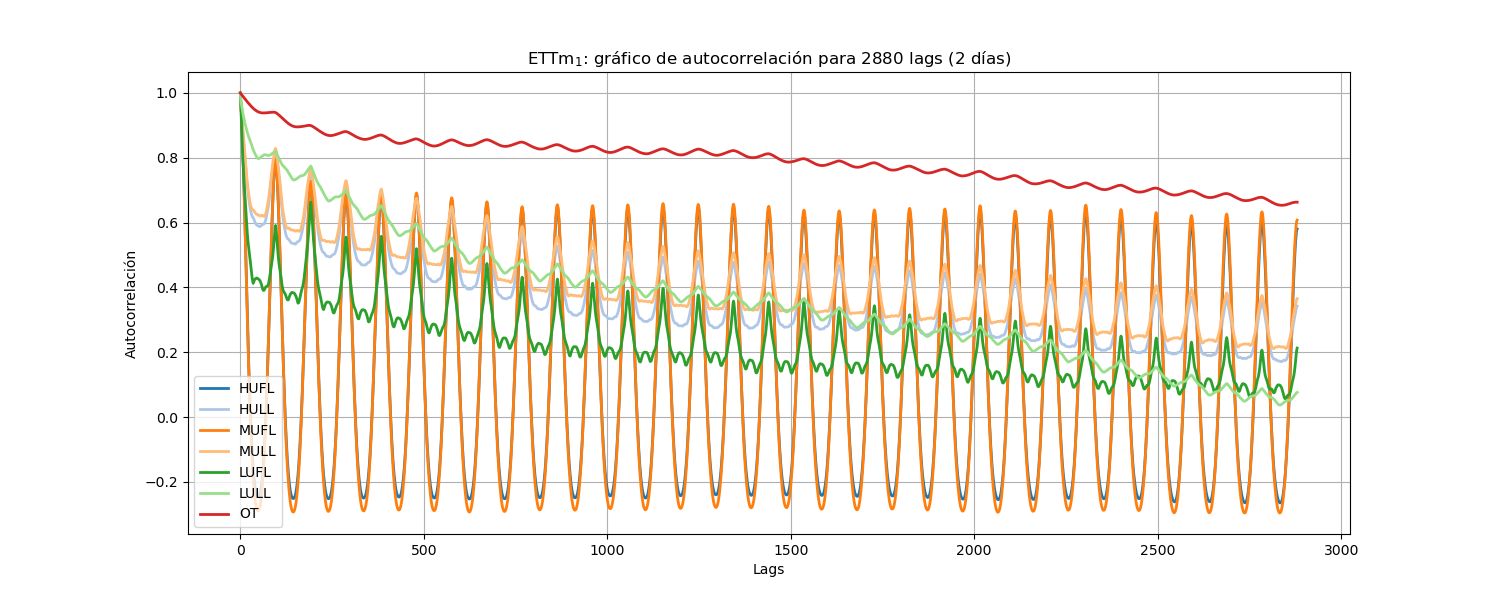
\includegraphics[scale=0.37]{img/etth1_autocorrelacion.png}
	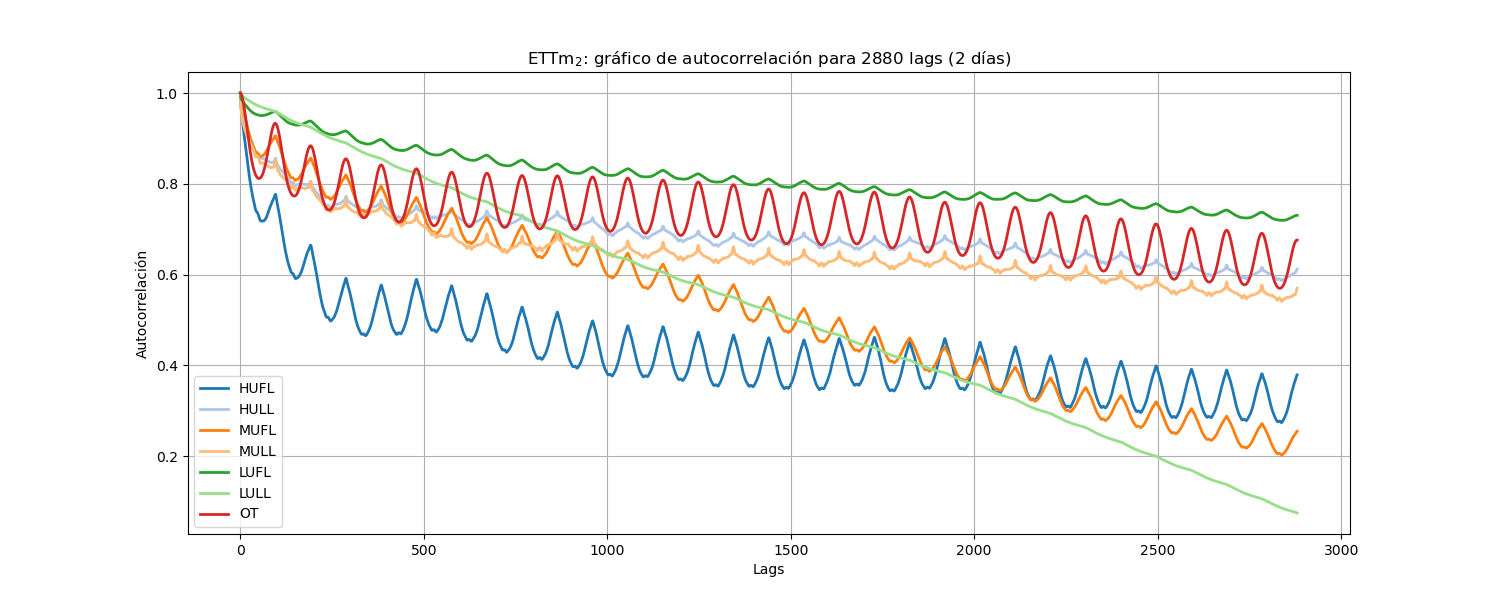
\includegraphics[scale=0.37]{img/etth2_autocorrelacion.png}
	\caption{ETT: gráficos de autocorrelación para ETTH$_1$ y ETTH$_2$}
	\label{autoett}
\end{figure}

En la figura \ref{autoett}, podemos apreciar el gráfico normalizado para las dos regiones, minuto a minuto, para una sucesión de 2880 lags, que equivale a una longitud de 2 días completos, para así observar información de estacionalidad a corto plazo.

\begin{itemize}
	\item Para el primer transformador, \textbf{ETTh1}, los valores parecen oscilar de manera considerable, pero muestran un comportamiento claramente estacional en todas sus variables. Si bien resulta complicado estimar el período concreto seguido, podemos ver claramente su evolución, y que no es una red estacionaria para ninguna de sus componentes. Por tanto, métodos clásicos como ARIMA no serían útiles, pero otros modelos más avanzados que sean capaces de recoger la semántica dada por cada estación nos permitiría obtener un buen rendimiento. A lo largo del tiempo, los valores de ACF prácticamente no varían, especialmente en carga media, cuyos valores ACF siempre oscilan en la misma amplitud y media. En cuanto a la correlación inmediata con el valor inmediatamente anterior, resulta ser bastante alta, por lo que podría ser una buena base para el modelado, pero sigue siendo necesario distinguir la estacionalidad para minimizar el error.
	\item En el caso de \textbf{ETTh2}, el comportamiento es algo diferente. Si bien la correlación con el anterior valor sigue siendo alta, y la estacionalidad se mantiene, la amplitud de los picos es bastante menor, indicando valores menos cambiantes y estables. Curiosamente, el comportamiento de \textit{LULL} contrasta bastante con el resto, ya que parece tener una tendencia claramente decreciente a cero. Sin embargo, para concocer la existencia de estacionalidad en dicha variable necesitaríamos ampliar demasiado el número de lags, y por tanto, dificultar el visualizado del resto de series. Basándonos en el otro transformador y las descripciones dadas de las variables, sí que se tratará de una serie también estacional, pero su período es de mayor amplitud y no apreciable.
\end{itemize}

En el caso de las variantes horarias, se trata simplemente de la misma información muestreada, por lo que el comportamiento será bastante similar al visto aquí pero con intervalos entre muestreos más largo (60 veces mayor exactamente).\\

De manera previa, a la vista de la información dada por los gráficos de autocorrelación, podemos intuir además de que el segundo conjunto puede ser más complejo de modelar, ya que además este no fue utilizado por el paper original de Informer ni buena parte de los modelos posteriores que se probaron. La mayoría optan por evaluar únicamente el primer transformador.

\section{Household Power Consumption (HPC)}

El siguiente dataset seleccionado a analizar es Household Power Consumption, un conjunto bastante extendido que puede ser encontrado en el repositorio UCI~\cite{hebrail2006individual}. Contiene la evolución del consumo eléctrico de una vivienda localizada cerca de París, entre los años 2006 y 2010, con el objetivo de poder construir un modelo capaz de representar el consumo asociado a dicha vivienda y sus diferentes sub-mediciones.\\

Continuamos de esta forma en el mismo ámbito que el dataset anterior, pero en este caso, nuestro objetivo no está centrado en evaluar el correcto funcionamiento del sistema, sino en ser capaces de modelar el consumo de la vivienda, y así poder realizar ajustes en la tarifa para contratar la potencia necesaria, o bien comprender el ciclo de consumo. Esta tarea es de vital importancia, ya que si escalamos su modelado a una población completa, podríamos obtener un modelo fiel capaz de ajustar los recursos eléctricos necesarios para su abastecimiento, y nos alineamos de nuevo con las necesidades de ahorro y eficiencia a la cual hemos dado importancia a lo largo de los diferentes ejemplos vistos en el trabajo.\\

Este dataset tiene su principal diferencia frente al anterior en su extensión. Nos encontramos ante un conjunto que ha sido recopilado de manera automatizada de un fenómeno real, con una frecuencia de muestreo de un minuto, y una extensión de 47 meses, entre diciembre de 2006 y noviembre de 2010, que nos aporta un total de 2,075,259 medidas. El número de variables muestreadas parece a priori superior, ya que en UCI se describe la existencia de 9 atributos, pero esto se debe realmente el timestamp ha sido separado en hora y fecha, pero si se unen, nos encontramos ante el mismo caso que ETT: cada instante de los datos consta de 8 características, incluyendo el timestamp y 7 variables de entrada.\\

Las variables recopiladas son las siguientes:

\begin{itemize}
	\item \textbf{date y time}. Son las variables asociadas a la fecha y hora en \textit{hh:mm:ss}, respectivamente. Ambas variables serán fusionadas más adelante en una sola columna para facilitar el procesado de los datos.
	
	\item \textbf{global\_active\_power}. Referido a la potencia activa global promedio por minuto del hogar (en kilovatios). Representa la energía eléctrica que se consume realmente para alimentar electrodomésticos, iluminación y otros dispositivos eléctricos.
	
	\item \textbf{global\_reactive\_power}. Potencia reactiva global promedio por minuto del hogar (en kilovatios). Esta potencia no realiza trabajo útil, sino que corresponde a la energía almacenada y liberada por componentes inductivos y capacitivos como motores o transformadores, afectando la eficiencia del sistema eléctrico a modo de pérdidas.
	
	\item \textbf{voltage}: Voltaje promedio por minuto (en voltios). Indica la diferencia de potencial eléctrico suministrada en el hogar.
	
	\item \textbf{global\_intensity}. Intensidad de corriente global promedio por minuto (en amperios). Mide la corriente eléctrica total que fluye en el sistema eléctrico de la vivienda y está directamente relacionada con el consumo.
	
	\item \textbf{sub\_metering\_1}: Se trata de una submedición de energía asociada a una región de la casa. En este caso, la número 1 (en vatios-hora de energía activa) corresponde a la cocina. En su publicación, podemos encontrar que esta medición incluye principalmente el lavavajillas, horno y microondas, pero no los fogones de la cocina, los cuales funcionan con gas y no mediante vitrocerámica.
	
	\item \textbf{sub\_metering\_2}: Submedición de energía número 2 (en vatios-hora de energía activa). En este caso, corresponde a la zona de lavandería, incluyendo la lavadora, secadora, frigorífico y una luz.
	
	\item \textbf{sub\_metering\_3}: Submedición de energía número 3 (en vatios-hora de energía activa). Corresponde al calentador eléctrico de agua y al aire acondicionado.
\end{itemize}

Una vez comprendida la semántica de cada variable del problema, podemos comenzar a hacer suposiciones sobre el conjunto de datos. Sabiendo que se trata de nuevo de un problema relacionado con la electricidad, es prácticamente evidente que podremos volver a encontrar patrones estacionales en muchas de las variables. Esto será potencialmente más notable en las submétricas extraídas, pero también en el resto de variables eléctricas. Por ejemplo, podremos encontrar patrones estacionales diarios en el uso de la submétrica 2, correspondiente a la cocina, ya que encontraremos momentos de mayor consumo asociados al horno y al microondas en horario de comidas; pero también la número 3, dado que se registran mayores consumos relacionados con el aire acondicionado en verano, así como un incremento en invierno debido al uso intensivo de agua caliente. Por tanto, es posible identificar un patrón con periodicidad anual, pero también patrones diarios asociados al uso de estos dispositivos: el agua caliente se utilizará principalmente en horarios relacionados con la higiene personal, mientras que el aire acondicionado se activa en las horas más calurosas del día.\\

Por tanto, los datos presentan estacionalidad a varios niveles, reflejando diferentes hábitos de consumo según la época y la hora del día, suponiendo así un buen benchmark para los positional encodings diseñados. Podemos verificarlo mediante un gráfico ACF (figura \ref{autohpc}), usando un período de nuevo de dos días de lags para así apreciar los picos de la señal.\\

\begin{figure}[!ht]
	\centering
	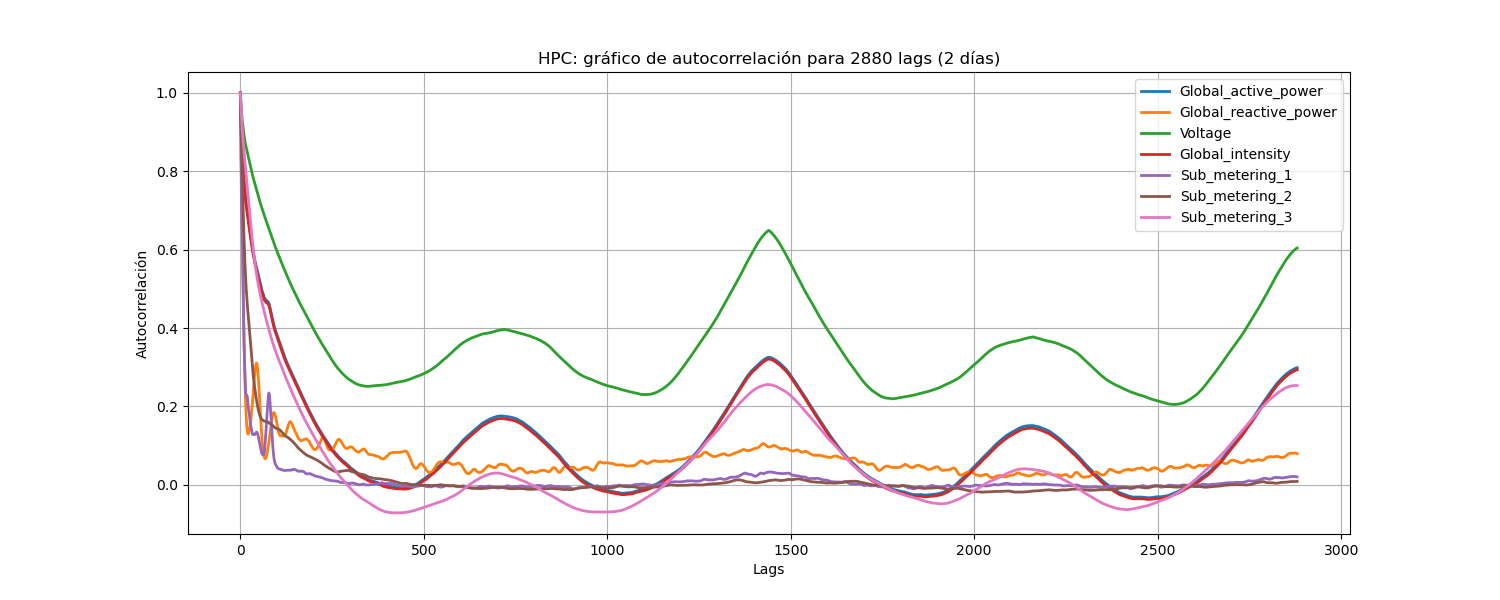
\includegraphics[scale=0.4]{img/hpc_autocorrelacion}
	\caption{HPC: gráfico de autocorrelación durante 2880 lags}
	\label{autohpc}
\end{figure}

Podemos apreciar varios fenómenos:
\begin{itemize}
	\item La variable \textit{voltage} tiene una oscilación considerable durante el día; podemos apreciar un valor mucho más elevado entorno a media noche (cada 1440 lags), mientras que este valor decae a lo largo del día (1440 lags con desfase de 1440), sufriendo un repunto más suave al mediodía. Esto puede estar asociado también a las exigencias que se da al sistema, ya que podemos ver que dichos puntos también coinciden con picos de intensidad global y consumo activo. Esto puede deberse a la propia forma de calcular potencia, como $P = I \cdot V$.
	\item Las variables \textit{global active power} y \textit{global intensity} están estrechamente relacionadas, hasta el punto de ser coincidentes en sus valores ACF, lo cual puede ser razonable teniendo en cuenta como se relacionaban ambas variables en el punto anterior.
	\item La variable de consumo pasivo, \textit{global reactive power} decae rápidamente a cero, y mantiene un comportamiento cercano a este durante práctica,ente toda la serie, al igual que las variables \textit{submetering 1 y 2}, que lo hacen de forma aún más cercana. Esto podría estar representando un comportamiento estacionario, ya que los valores de ACF decaen rápidamente, por lo que modelar dichas variables con métodos más sencillos como ARIMA sería viable en caso de que se requiriese, dada la escasa variabilidad a lo largo del tiempo. 
	\item El área 3, \textit{submetering 3}, es la que presenta un comportamiento estacional, a diferencia de las otras 2 sub divisiones de la vivienda. Esto se debe principalmente a la necesidad de agua caliente para higiene de manera periódica y la climatización, como ya mencionamos anteriormente.
\end{itemize}

Por tanto, el análisis de la autocorrelación nos ha aportado información muy valiosa acerca del problema: tenemos tanto variables estacionales, como componentes aparentemente estacionarias en el tiempo, aportando bastante complejidad al modelo, que tendrá que adaptarse a todo ello, y la codificación posicional cobrará importancia.

\subsection{Yellow Trip Data}

El tercer dataset a evaluar será Yellow Trip Data, cuya temática diverge del tema energético visto hasta el momento para estudiar nuevas semánticas de problemas. Este conjunto de datos podemos encontrarlo en la web de New York City Open Data~\cite{nycopendata}, donde se alojan multitud de datos públicos actualizados anualmente de diferentes sistemas de la ciudad. Basados en datos del año 2015, esta variante ha sido expandida artificialmente para aumentar el tamaño de la serie hasta sobrepasar las 2 millones de instancias.\\

El conjunto de datos contiene información sobre los viajes realizados mediante el servicio de taxi en la ciudad de Nueva York, con el propósito de modelar los patrones de comportamiento de los usuarios durante sus desplazamientos. Desde un enfoque analítico, estimar la demanda del servicio y la duración de los viajes resulta fundamental para optimizar la asignación de vehículos en circulación, evitando la existencia de conductores ociosos y contribuyendo a la reducción del tráfico en la ciudad. De este modo, no solo se mejora la fluidez vehicular, sino que también se disminuye el consumo energético y las emisiones contaminantes al eliminar vehículos innecesarios.\\

Aunque a nivel estructural este conjunto de datos presenta una dimensionalidad similar a la de HPC, al estar muestreado de forma horaria y haber sido ampliado artificialmente, cubre un período temporal considerablemente mayor, cercano a los 254 años. Además, dado que en el transcurso de una hora pueden realizarse cientos de viajes de distintos vehículos, los datos han sido agrupados, lo que se refleja en valores elevados en cada una de las variables. La dimensionalidad para cada instante también cambia: además del timestamp, se dispone de otras 6 variables, reduciendo así en una dimensión el problema.\\

Las variables recogen la siguiente información:

\begin{itemize}
	\item \textbf{passenger\_count}. Número de pasajeros que viajaron en el trayecto. Recoge la ocupación total en una hora, y podría extraerse valores como la media y su impacto en el ingreso generado.
	
	\item \textbf{trip\_distance}. Distancia recorrida durante el viaje, medida en millas. De este atributo podemos evaluar patrones de movilidad y relacionar la distancia con el momento temporal.
	
	\item \textbf{fare\_amount}. Precio base de la tarifa cobrada por el viaje, sin incluir impuestos, propinas u otros cargos adicionales. Refleja el coste inicial calculado según distancia y tiempo.
	
	\item \textbf{tip\_amount}. Propina pagada al conductor. Es un indicador del nivel de satisfacción del pasajero y también afecta los ingresos totales del conductor, y resulta interesante estudiar para ver si depende del momento del día o la época del año.
	
	\item \textbf{total\_amount}. Cantidad total pagada por el pasajero, incluyendo tarifa base, impuestos, propinas, peajes y cualquier otro cargo extra. Representa, por tanto, el ingreso final recibido por el servicio.
	
	\item \textbf{trip\_duration}. Duración del viaje, expresada en minutos. Permite analizar la eficiencia y velocidad promedio del trayecto, así como detectar posibles congestiones o retrasos en el tráfico.
\end{itemize}

Existen otras variables recogidas por el conjunto de datos, como método de pago, modelo del vehículo, y otra información adicional de contenido no numérico que ha sido desestimada, debido a que no sería posible entonces agrupar los viajes por hora si intervienen factores no acumulables cuantitativamente.\\

A priori, tan solo examinando las variables numéricas seleccionadas y su descripción, ya podemos apreciar patrones claros que describirá el conjunto de datos. Por ejemplo, la distancia de los viajes posiblemente será mayor en verano debido posiblemente al efecto del turismo, pero menor en las primeras horas del día, aunque con mayor duración debido a los atascos; en el caso de los ocupantes, potencialmente también tendrá mayores extremos en meses turísticos del año, como Navidad. O bien, si nos fijamos en el coste total, este será potencialmente mayor en horario nocturno. Todos estos comportamientos podremos examinarlos de forma aproximada si volvemos a recurrir al gráfico de autocorrelaciones (figura  \ref{autotaxi}).\\
	
\begin{figure}[!ht]
	\centering
	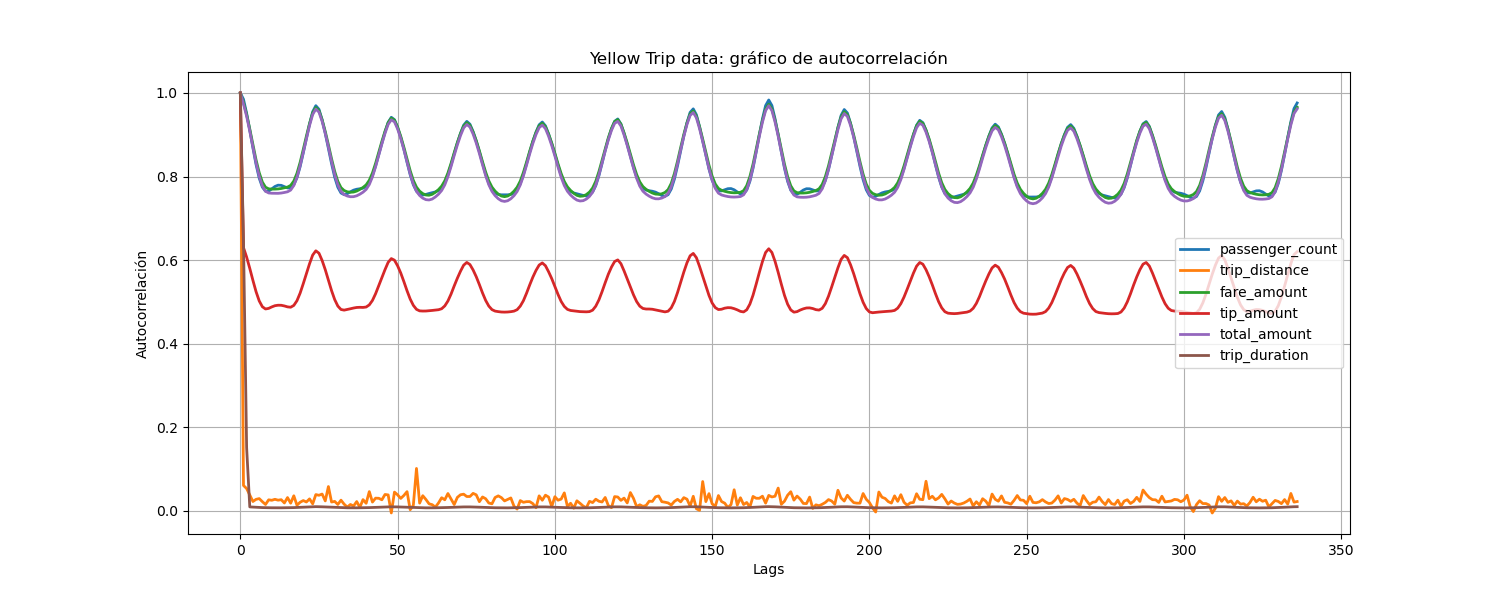
\includegraphics[scale=0.4]{img/taxi_autocorrelacion}
	\caption{Yellow Trip data: gráfico de autocorrelación durante 336 lags}
	\label{autotaxi}
\end{figure}
	
En este caso, lo analizaremos durante 336 lags, el equivalente a 2 semanas de tiempo:

\begin{itemize}
	\item La variable \textit{trip distance} parece decaer rápidamente en sus valores de correlación hasta el valor cero. Esto indica una gran relación con el valor posterior, y la disminución temprana de los valores indica que estamos potencialmente ante una variable estacionaria. Esto quiere decir que, posiblemente, la distancia media de los viajes no se ve afectada por las variables de tiempo en gran medida.
	\item Existe una gran relación entre el \textit{passenger count} y el precio base (\textit{fare amount}) de los viajes. Esto tiene sentido, ya que a un mayor número de pasajeros por hora, se habrá realizado un mayor número de carreras, y por tanto, aumentan los ingresos. En ambas variables se puede apreciar además un claro patrón estacional de entorno a 15 horas, marcando así mediante los valores máximos los momentos de inicio y fin de jornada laboral, tal y como intuíamos.
	\item \textit{tip amount}, la variable asociada a las propinas, parece tener un comportamiento bastante sincronizado con las dos variables anteriores: los picos máximos coinciden con los momentos de mayor traslado de personas, lo cual es probabilísticamente razonable, ya que a mayor cantidad de viajeros, mayor probabilidad también de recibir propina.
\end{itemize}

En definitiva, aunque este conjunto de datos presenta un menor número de atributos que los anteriores, su comportamiento es bastante similar: incluye variables estacionales y estacionarias, lo que añade complejidad al proceso de entrenamiento, y resulta adecuado como \textit{benchmark}. No obstante, dado que ha sido ampliado artificialmente, es posible que contenga valores anómalos, especialmente en los tramos finales de la serie, por lo que los resultados deben interpretarse con espíritu crítico.

\section{Time-series Industrial Anomaly dataset (TINA)}

Por último, presentamos el conjunto de datos \textit{Time-series Industrial Anomaly} (TINA)~\cite{tina_dasci_arcelor}, publicado en la web de DASCI y orientado al análisis de series temporales para la detección de anomalías en entornos industriales. Este conjunto fue construido a partir de información recopilada por sensores instalados en una máquina de minería perteneciente a la compañía ArcelorMittal. En su formato original, fue muestreado en intervalos de 2 segundos, abarcando el período comprendido entre el 6 de septiembre de 2017 y el 25 de diciembre de 2018, lo que resulta en aproximadamente 38 millones de instancias. Su construcción se ha realizado uniendo diferentes ficheros de datos correspondientes a cada día de uso de la máquina, por lo que, su peso asciende a varias decenas de GB de información.\\

Resulta complejo analizar la semántica del problema, ya que este conjunto fue convenientemente anonimizado para evitar filtrar datos sensibles de la empresa. Además, han sido normalizadas, por lo que todos los valores se encuentran en el mismo intervalo. En total, se dispone de 108 columnas, las cuales pueden ser tanto de naturaleza numérica como categórica, siguiendo la notación ``FEATURE n'', donde n es el número de atributo, desde 0 hasta 107. Concretamente, las columnas categóricas de este conjunto de datos son:

\begin{itemize}
	\item \texttt{FEATURE76} y \texttt{FEATURE87}. Son variables categóricas cuyo significado específico no se detalla en la fuente de datos.
	\item \texttt{m\_id}. Indica la existencia o ausencia de un mantenimiento en un instante temporal determinado, codificando el tipo de mantenimiento mediante un identificador numérico. Un mantenimiento implica la detención completa de la máquina; por ello, la operación normal no se restablece inmediatamente tras su finalización, debido al tiempo de recuperación que el propio sistema requiere.
	\item \texttt{m\_subid}. Especifica el subtipo de mantenimiento, en caso de haberse producido.
	\item \texttt{alarms}. Señala la ocurrencia de eventos de alarma.
\end{itemize}



Debido a la elevada dimensionalidad del conjunto de datos, la ejecución directa de pruebas con los distintos encodings resulta compleja, ya que si recordamos, la mayoría de las alternativas propuestas por los métodos de ventana dependen tanto de la longitud $L$, como del número de atributos $d$. Por ello, hemos decidido revisar y ajustar ciertos aspectos antes de proceder con las evaluaciones:

\begin{itemize}
	\item Se han descartado todas las variables categóricas, ya que, al ser anónimas, no aportan información semántica relevante al problema y su codificación supondría un coste computacional elevado sin una ganancia clara en el rendimiento del modelo.
	\item Por otro lado, dado que los 38 millones de instancias originales pueden sobrepasar la capacidad de memoria de cualquier GPU doméstica e incluso de algunas profesionales, se ha optado por reducir el muestreo a intervalos de 30 segundos. Esta medida disminuye significativamente el tamaño del conjunto de datos, pasando a aproximadamente 2,5 millones de instancias, lo que hace el proceso de entrenamiento mucho más manejable. Consideramos que se trata de un este intervalo equilibrado, ya que permite conservar la estructura temporal y los patrones relevantes para la detección de anomalías, reduciendo la pérdida de información.
\end{itemize}

De esta forma, disponemos de un conjunto de datos variado y de mayor complejidad, capaz de valorar el correcto funcionamiento de las codificaciones no sólo en longitud de secuencia, sino también en anchura de la misma. Todo ello, ajustándonos a los recursos disponibles tratando de minimizar la pérdida de información. Su inclusión en el conjunto de datos de evaluación de estos, además, nos motiva a implementar procedimientos de forma eficiente, ya que, sin una adecuada escalabilidad, la ejecución sobre este dataset sería inviable. Incluso la simple generación del gráfico de autocorrelación, mediante el paquete \textit{statsmodels}, con el objetivo de identificar patrones visuales en los datos, provoca problemas de desbordamiento de memoria. Por ello, en este conjunto de datos concreto se ha optado por prescindir de su graficado, y por desgracia, podremos depende únicamente de los resultados experimentales para realizar el análisis.



